\documentclass{article}
\usepackage[margin=0.9in]{geometry}
\usepackage{amsmath}
\usepackage{amssymb}
\usepackage{booktabs}
\usepackage{xintexpr}
\usepackage{tikz}
\usetikzlibrary{arrows,automata}
\usepackage{subcaption}
\usepackage{float}
\usepackage{fancyhdr}

\pagestyle{fancy}
\lhead{Tanner Hobson}
\rhead{thobson2}

\newcommand{\T}{1}
\newcommand{\F}{0}
\newcommand{\TF}[1]{\if1#1\T\else\F\fi}
\newcommand{\xintTF}[1]{\xintifboolexpr{#1}{\T}{\F}}

\newcommand{\logicrule}[2]{
\begin{array}{l}
#1 \\
\midrule
\therefore #2 \\
\end{array}
}

\newcommand{\inv}[1]{#1^{-1}}

\renewcommand{\d}[1]{\,\textnormal{d}#1}
\newcommand{\dd}[2]{\frac{\d{#1}}{\d{#2}}}
\newcommand{\ddd}[2]{\dfrac{\d{#1}}{\d{#2}}}

\DeclareMathOperator{\var}{Var}
\DeclareMathOperator{\E}{\mathcal{E}}

\newcommand{\multistep}[1]{\begin{array}{rl} #1 \end{array}}
\newcommand{\subeq}{\subseteq}
\newcommand{\sub}{\subset}

\newcommand{\conj}[1]{\overline{#1}}

\newcommand{\problem}[1]{$\boxed{\textbf{#1}}$}

\setlength\parindent{0pt}
\setlength\parskip{0em}

\begin{document}

\begin{minipage}{\textwidth}
\problem{3.1}

\begin{figure}[H]
  \centering
  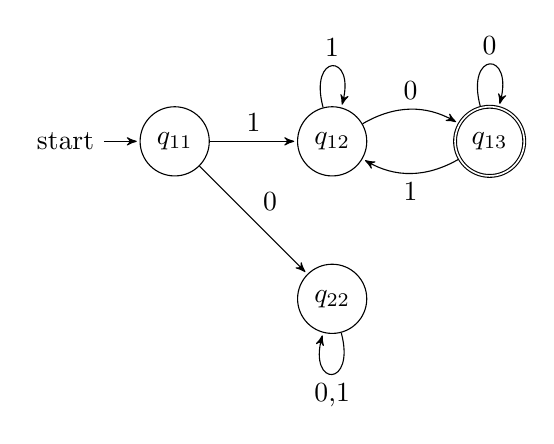
\begin{tikzpicture}[>=stealth',shorten >=1pt,auto,node distance=2cm]
    \node[initial,state] (q11) {$q_{11}$};
    \node[state] (q12) [right of=q11] {$q_{12}$};
    \node[state,accepting] (q13) [right of=q12] {$q_{13}$};
    \node[state] (q22) [below of=q12] {$q_{22}$};

    \path[->]
    (q11) edge node {0} (q22)
    (q11) edge node {1} (q12)

    (q12) edge [bend left] node {0} (q13)
    (q12) edge [loop above] node {1} (q12)

    (q13) edge [loop above] node {0} (q13)
    (q13) edge [bend left] node {1} (q12)

    (q22) edge [loop below] node {0,1} (q22)
    ;
  \end{tikzpicture}
  \caption{$M_1$}
\end{figure}
\end{minipage}

\begin{minipage}{\textwidth}
\problem{3.2}

\begin{figure}[H]
  \centering
  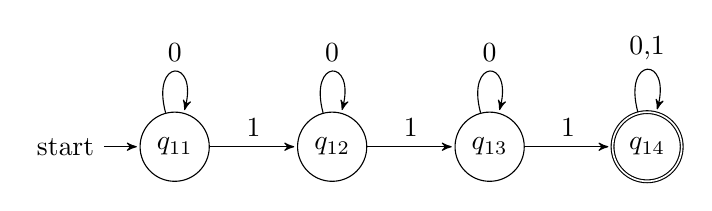
\begin{tikzpicture}[>=stealth',shorten >=1pt,auto,node distance=2cm]
    \node[initial,state] (q11) {$q_{11}$};
    \node[state] (q12) [right of=q11] {$q_{12}$};
    \node[state] (q13) [right of=q12] {$q_{13}$};
    \node[state,accepting] (q14) [right of=q13] {$q_{14}$};

    \path[->]
    (q11) edge [loop above] node {0} (q11)
    (q11) edge node {1} (q12)

    (q12) edge [loop above] node {0} (q12)
    (q12) edge node {1} (q13)

    (q13) edge [loop above] node {0} (q13)
    (q13) edge node {1} (q14)

    (q14) edge [loop above] node {0,1} (q14)
    ;
  \end{tikzpicture}
  \caption{$M_2$}
\end{figure}
\end{minipage}

\begin{minipage}{\textwidth}
\problem{3.3}

\begin{figure}[H]
  \centering
  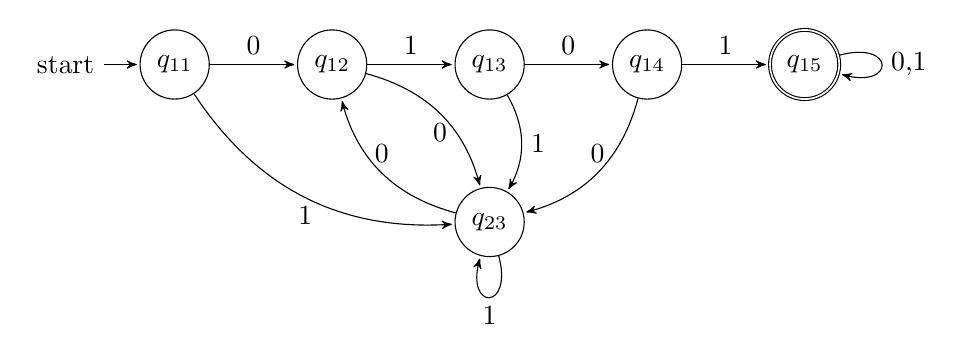
\begin{tikzpicture}[>=stealth',shorten >=1pt,auto,node distance=2cm]
    \node[initial,state] (q11) {$q_{11}$};
    \node[state] (q12) [right of=q11] {$q_{12}$};
    \node[state] (q13) [right of=q12] {$q_{13}$};
    \node[state] (q14) [right of=q13] {$q_{14}$};
    \node[state,accepting] (q15) [right of=q14] {$q_{15}$};
    \node[state] (q23) [below of=q13] {$q_{23}$};

    \path[->]
    (q11) edge node {0} (q12)
    (q11) edge [bend right] node [below] {1} (q23)

    (q12) edge [bend left] node [below] {0} (q23)
    (q12) edge node {1} (q13)

    (q13) edge node {0} (q14)
    (q13) edge [bend left] node {1} (q23)

    (q14) edge [bend left] node [above] {0} (q23)
    (q14) edge node {1} (q15)

    (q15) edge [loop right] node {0,1} (q15)

    (q23) edge [bend left] node [above] {0} (q12)
    (q23) edge [loop below] node {1} (q23)
    ;
  \end{tikzpicture}
  \caption{$M_3$}
\end{figure}
\end{minipage}

\begin{minipage}{\textwidth}
\problem{3.4}

\begin{figure}[H]
  \centering
  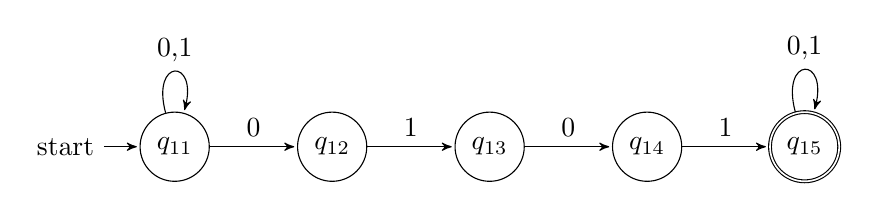
\begin{tikzpicture}[>=stealth',shorten >=1pt,auto,node distance=2cm]
    \node[initial,state] (q11) {$q_{11}$};
    \node[state] (q12) [right of=q11] {$q_{12}$};
    \node[state] (q13) [right of=q12] {$q_{13}$};
    \node[state] (q14) [right of=q13] {$q_{14}$};
    \node[state,accepting] (q15) [right of=q14] {$q_{15}$};

    \path[->]
    (q11) edge [loop above] node {0,1} (q11)
    (q11) edge node {0} (q12)

    (q12) edge node {1} (q13)

    (q13) edge node {0} (q14)

    (q14) edge node {1} (q15)

    (q15) edge [loop above] node {0,1} (q15)
    ;
  \end{tikzpicture}
  \caption{$M_4$}
\end{figure}
\end{minipage}

\begin{minipage}{\textwidth}
\problem{3.5}

We start with $Q=\varnothing$.

Then we add the initial state of the NFA to $Q$, and therefore we have
$Q=\{\{1\}\}$.

Then we let $q=\{1\}$ and find that $\delta_2(1,a)=\{1,2\}$ and
therefore $\delta(\{1\},a)=\{1,2\}$. Similarly, we find
$\delta_2(1,b)=\{2\}$ and conclude that
$\delta(\{1\},b)=\{2\}$. Finally, we add $\{1,2\}$ and $\{2\}$ to $Q$,
giving $Q=\{\{1\},\{1,2\},\{2\}$.

Now we let $q=\{1,2\}$ and recall that $\delta_2(1,a)=\{1,2\}$ and
find $\delta_2(2,a)=\varnothing$. Additionally, we find
$\delta_2(1,b)=\{2\}$ and $\delta_2(2,b)=\{1\}$. From this we can add
$\varnothing\cup\{\{1,2\}\}=\{\{1,2\}\}$ and
$\{\{2\}\}\cup\{\{1\}\}=\{\{1\},\{2\}\}$ to $Q$, giving
$Q=\{\{1\},\{1,2\},\{2\}\}$.

Now we let $q=\{2\}$ and find that $\delta_2(2,a)=\varnothing$ and
$\delta_2(2,b)=\{1\}$. We then add $\{\varnothing\}$ and $\{\{1\}\}$
to $Q$, giving $Q=\{\varnothing,\{1\},\{2\},\{1,2\}\}$.

Now we know that our nodes are $\{1\}$, $\{2\}$, and $\{1,2\}$.

%\begin{figure}[H]
%  \centering
%  \begin{tikzpicture}[>=stealth',shorten >=1pt,auto,node distance=2cm]
%    \node[initial,state] (q11) {$\{1\}$};
%    \node[state] (q12) [right of=q11] {$\{1,2\}$};
%    \node[state] (q13) [right of=q12] {$\{2\}$};
%    \node[state] (q22) [below of=q12] {$\varnothing$};
%
%    \path[->]
%    (q11) edge node {a} (q12)
%    (q11) edge node {b} (q13)
%
%    (q12) edge [loop above] node {a,b} (q12)
%    ;
%  \end{tikzpicture}
%  \caption{$M_4$}
%\end{figure}
\end{minipage}

\end{document}
